\documentclass{standalone}
\usepackage{tikz}
\usepackage{amsmath}
\usepackage{bm}
\usetikzlibrary{decorations.pathmorphing,arrows.meta}

\begin{document}

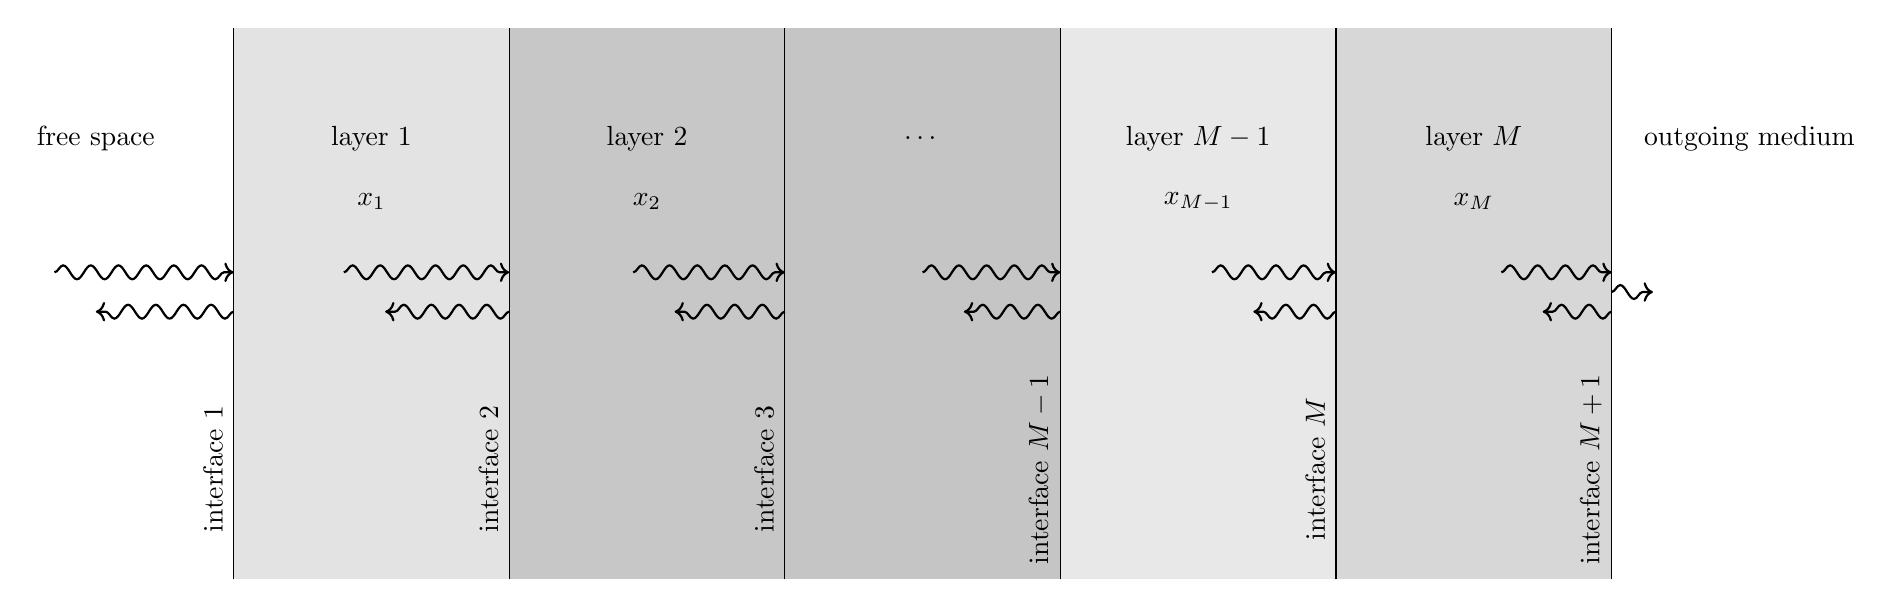
\begin{tikzpicture}

% Define the colors for the background boxes
\definecolor{lightgray}{gray}{0.9}

% Box coordinates and dimensions
\def\boxwidth{3.5cm}
\def\boxheight{3.5cm}
\def\centerheight{-0.1cm}

% Draw the main boxes with alternating colors
\pgfmathsetseed{1254}
\foreach \i in {1,2,3,4,5} {
    \pgfmathsetmacro{\shade}{20 + 40*rand} % gives something between gray!10 and gray!30
    \node[
        fill=gray!\shade,
        minimum width=\boxwidth,
        minimum height=2*\boxheight
    ] at (\i * \boxwidth, 0) {};
}
\foreach \i in {1,2,3,4,5,6} {
    \draw (\i * \boxwidth - 0.5* \boxwidth, -\boxheight) -- (\i * \boxwidth - 0.5 * \boxwidth, \boxheight);
}

% Add labels inside each box
\node at (1*\boxwidth, 1.3) {$x_1$};
\node at (2*\boxwidth, 1.3) {$x_2$};
% \node at (3*\boxwidth, 0.9) {$...$};
\node at (4*\boxwidth, 1.3) {$x_{M-1}$};
\node at (5*\boxwidth, 1.3) {$x_M$};


% Draw horizontal arrows inside each box
\foreach \i in {0,1,2,3,4,5} {
    % \draw[->] (\i*\boxwidth + 0.25*\boxwidth, \centerheight + 0.5cm) -- (\i*\boxwidth + 0.5*\boxwidth, \centerheight + 0.5cm);
    \draw[
    decorate,
    decorate,decoration={snake,post length=1mm},
    ->,
    thick
    ]
    (\i*\boxwidth + \i*0.05*\boxwidth - 0.15*\boxwidth, \centerheight + 0.5cm)
    -- (\i*\boxwidth + 0.5*\boxwidth, \centerheight + 0.5cm);
    \draw[    
        decorate,
    decorate,decoration={snake,post length=1mm},
    ->,
    thick
    ] 
    (\i*\boxwidth + 0.5*\boxwidth, \centerheight) -- (\i*\boxwidth + \i*0.05*\boxwidth, \centerheight);
}
\draw[   
    decorate,
    decorate,decoration={snake,post length=1mm},
    ->,
    thick
]
(5.5*\boxwidth, \centerheight + 0.25cm) -- (5.65*\boxwidth, \centerheight + 0.25cm);

% Label arrows
% \node at (0.15*\boxwidth, -0.3) {$E_{1,\pm}^f$};
% \node at (1.15*\boxwidth, -0.3) {$E_{2,\pm}^f$};
% \node at (2.15*\boxwidth, -0.3) {$E_{3,\pm}^f$};
% \node at (3.15*\boxwidth, -0.3) {$...$};
% \node at (4.15*\boxwidth, -0.3) {$E_{M,\pm}^f$};
% \node at (5.05*\boxwidth, -0.3) {$E_{M+1,\pm}^f$};

% \node at (0.15*\boxwidth, \centerheight-0.3cm) {$E_{1,-}^f$};
% \node at (1.15*\boxwidth, \centerheight-0.3cm) {$E_{2,-}^f$};
% \node at (2.15*\boxwidth, \centerheight-0.3cm) {$E_{3,-}^f$};
% \node at (3.15*\boxwidth, \centerheight-0.3cm) {$...$};
% \node at (4.15*\boxwidth, \centerheight-0.3cm) {$E_{M,-}^f$};
% \node at (5.15*\boxwidth, \centerheight-0.3cm) {$E_{M+1,-}^f$};
% \node at (0.15*\boxwidth, \centerheight+0.6cm) {$E_{1,+}^f$};
% \node at (1.15*\boxwidth, \centerheight+0.6cm) {$E_{2,+}^f$};
% \node at (2.15*\boxwidth, \centerheight+0.6cm) {$E_{3,+}^f$};
% \node at (3.15*\boxwidth, \centerheight+0.6cm) {$...$};
% \node at (4.15*\boxwidth, \centerheight+0.6cm) {$E_{M,+}^f$};
% \node at (5.15*\boxwidth, \centerheight+0.6cm) {$E_{M+1,+}^f$};

% Top labels for slabs and free space
\node at (0.*\boxwidth, 2.1) {free space};
\node at (1.*\boxwidth, 2.1) {layer $1$};
\node at (2.*\boxwidth, 2.1) {layer $2$};
\node at (3.*\boxwidth, 2.1) {$\dots$};
\node at (4.*\boxwidth, 2.1) {layer $M-1$};
\node at (5.*\boxwidth, 2.1) {layer $M$};
\node at (6.*\boxwidth, 2.1) {outgoing medium};

% Bottom labels for E
\node[rotate=90] at (0.425*\boxwidth, -2.1) {interface $1$};
\node[rotate=90] at (1.425*\boxwidth, -2.1) {interface $2$};
\node[rotate=90] at (2.425*\boxwidth, -2.1) {interface $3$};
% \node[rotate=90] at (2.8*\boxwidth, -2.1) {$...$};
\node[rotate=90] at (3.425*\boxwidth, -2.1) {interface $M-1$};
\node[rotate=90] at (4.425*\boxwidth, -2.1) {interface $M$};
\node[rotate=90] at (5.425*\boxwidth, -2.1) {interface $M+1$};


% % Add rho labels under boxes
% \foreach \i/\label in {1/\rho_1, 2/\rho_2, 3/\rho_3, 4/\rho_4, 5/\rho_{\textit{i}}, 6/\rho_{\textit{i}+1}, 7/\rho_M} {
%     \node at (\i*\boxwidth, -0.6) {$\label$};
% }

\end{tikzpicture}

\end{document}
